%2020年 09月 22日 星期二 22:27:06 CST
\documentclass[a4paper,fontset = windows]{ctexbook}
\usepackage[margin=2cm]{geometry}
\usepackage{xifthen}
\usepackage{calc}
\usepackage{graphicx}
\usepackage{tikz}
\usetikzlibrary{patterns}
\usepackage{amsmath}
\usepackage{amsfonts}
\usepackage{amssymb}
\usepackage{cexam}
\usepackage{xcolor}

\begin{document}
\chapter{图片与文字分离升级程序}
此处为了解决一个文件中有多个图片时,并列排版的问题。

\subsection{例题分析}
\begin{jisuan}[example]

%2020年 09月 24日 星期四 00:28:05 CST
% have a bug 
 e.物体静止则受力平衡,所以重力与竖直绳的拉力平衡,则竖直绳的拉力大小$F=G$.由于绳的拉力一定沿绳指向绳收缩的方向,铰链所受力的方向一定沿杆的方向.所以得出力分解的两个效果的方向就是绳收缩的方向和杆压缩的方向.由此作平行四边形如
 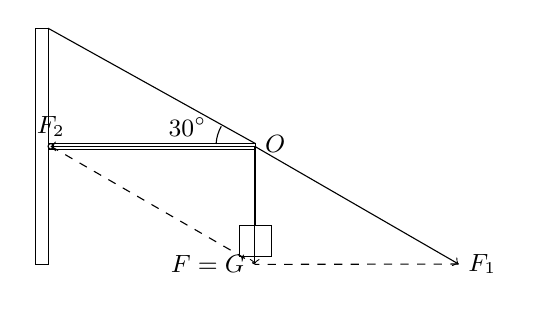
\begin{tikzpicture}
   \draw (-0.2,1.5) rectangle (-1pt,-1.5);
   \draw (0,0) circle [radius=1pt];
   \draw (-1pt,-1pt) rectangle (2.598,1pt) node [anchor=west]{\small $O$};
   \draw (-1pt,1.5) -- (2.598,1pt);
   \draw (2.598,1pt)--(2.598,-1);
   \draw (2.398,-1) rectangle (2.798,-1.4);
   \draw (2.165,0.254) arc (150:177:0.5);
   \draw (2.098,0) node [anchor=south east]{\small $30^\circ$};
   \draw [->](2.589,0)--(0,0) node [anchor=south]{\small $F_2$};
   \draw [->](2.589,0)--(2.589,-1.4948) node [anchor=east] {\small $F=G$};
   \draw [->](2.589,0)--(5.178,-1.4948) node [anchor=west] {\small $F_1$};
   \draw [dashed] (0,0)--(2.589,-1.4948);
   \draw [dashed] (5.178,-1.4948)--(2.589,-1.4989);
 \end{tikzpicture}
 所示,由几何关系得所示,由几何关系得
 $$F_1=\cfrac{G}{\sin\theta}=60N,F_2=\cfrac{G}{\tan\theta}\approx 52N$$

 \end{jisuan}

\end{document}
